\chapter{Data Aggregation Background} % (fold)
\label{cha:Data Aggregation Background}

One of the fundamental and indispensable functionalities of sensor networks
is the ability to answer queries over the data acquired by the
sensors. 
For example, in Figure \ref{fig:Routing River} the base station might be at the end of the river who initiates the query to the sensor network.
And all the sensor nodes on both sides of the river has to response to the queries of the base station.
\begin{figure}[h!]
	\centering
	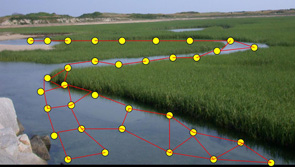
\includegraphics[scale = 2]{images/routing-river.jpg}\\
	\caption{Routing River \cite{RoutingRiver}}
	\label{fig:Routing River}
\end{figure}

The resource constraints and security issues make designing mechanisms for information aggregation in large sensor networks particularly challenging.

Literature survey on data aggregation
	
	Read SIA; you can take inspiration from it for SIA

	talk about compression

	lossy compression

	lossless compression

	data aggregation is lossy compression as there is no way the base station can know the original sensor readings 

	Hence, confidence in data is so important.

then talk about SHIA